%%%%%%%%%%%%%%%%%%%%%%%%%%%%%%%%%%%%%%%%%%%%%%%%%%%%%%%%%%%%%%%%%%%%%%
% LaTeX Template: Newsletter  % Source: http://www.howtotex.com
%
% Feel free to distribute this example, but please keep the referral
% to howtotex.com
% Date: September 2011 
% 
%%%%%%%%%%%%%%%%%%%%%%%%%%%%%%%%%%%%%%%%%%%%%%%%%%%%%%%%%%%%%%%%%%%%%%
% How to use writeLaTeX: 
%
% You edit the source code here on the left, and the preview on the
% right shows you the result within a few seconds.
%
% Bookmark this page and share the URL with your co-authors. They can
% edit at the same time!
%
% You can upload figures, bibliographies, custom classes and
% styles using the files menu.
%
% If you're new to LaTeX, the wikibook is a great place to start:
% http://en.wikibooks.org/wiki/LaTeX
%
%%%%%%%%%%%%%%%%%%%%%%%%%%%%%%%%%%%%%%%%%%%%%%%%%%%%%%%%%%%%%%%%%%%%%%
% Edit the title below to update the display in My Documents
%\title{Edukasyon Sa Pagpapakatao 7}

%%% ---------------
%%% PREAMBLE
%%% ---------------
\documentclass[10pt,a4paper]{article}

% Define geometry (without using the geometry package)
\setlength\topmargin{-48pt}
\setlength\headheight{0pt}
\setlength\headsep{25pt}
\setlength\marginparwidth{-20pt}
\setlength\textwidth{7.0in}
\setlength\textheight{9.5in}
\setlength\oddsidemargin{-30pt}
\setlength\evensidemargin{-30pt}

\frenchspacing						% better looking spacing

% Call packages we'll need
\usepackage[english]{babel}			% english
\usepackage{graphicx}				% images
\usepackage{amssymb,amsmath}		% math
\usepackage{multicol}				% three-column layout
\usepackage{url}					% clickable links
\usepackage{marvosym}				% symbols
\usepackage{wrapfig}				% wrapping text around figures
\usepackage[T1]{fontenc}			% font encoding
\usepackage{charter} 				% Charter font for main content
\usepackage{blindtext}				% dummy text
\usepackage{datetime}				% custom date
	\newdateformat{mydate}{{June} \THEYEAR}
\usepackage[pdfpagemode=FullScreen,
			colorlinks=false]{hyperref}	% links and pdf behaviour

% Customize (header and) footer
\usepackage{fancyhdr}
\pagestyle{fancy}
\lfoot{	\footnotesize 
		Edukasyon Sa Pagpapakatao 7-Modyul 1\\
				\Letter\ \href{mailto:daniloblancojr0731@gmail.com}{daniloblancojr0731@gmail.com}
	  }
\cfoot{}
\rfoot{\footnotesize ~\\ Page \thepage}
\renewcommand{\headrulewidth}{0.0pt}	% no bar on top of page
\renewcommand{\footrulewidth}{0.4pt}	% bar on bottom of page

%%% ---------------
%%% DEFINITIONS
%%% ---------------

% Define separators
\newcommand{\HorRule}[1]{\noindent\rule{\linewidth}{#1}} % Creating a horizontal rule
\newcommand{\SepRule}{\noindent							 % Creating a separator
						\begin{center}
							\rule{250pt}{1pt}
						\end{center}
						}						

% Define Title en News input
\newcommand{\JournalName}[1]{%
		\begin{center}	
			\Huge \usefont{T1}{augie}{m}{n}
			#1%
		\end{center}	
		\par \normalsize \normalfont}
		
\newcommand{\JournalIssue}[1]{%
		\hfill \textsc{\mydate \today, No #1}
		\par \normalsize \normalfont}

\newcommand{\NewsItem}[1]{%
		\usefont{T1}{augie}{m}{n} 	
		\large #1 \vspace{4pt}
		\par \normalsize \normalfont}
		
\newcommand{\NewsAuthor}[1]{%
			\hfill by \textsc{#1} \vspace{4pt}
			\par \normalfont}		


%%% ---------------
%%% BEGIN DOCUMENT
%%% ---------------
\begin{document}
% Title	
% -----
\JournalIssue{1}
\JournalName{Edukasyon Sa Pagpapakatao 7}
\noindent\HorRule{3pt} \\[-0.75\baselineskip]
\HorRule{1pt}
% -----

% Front article
% -----
\vspace{0.5cm}
	\SepRule
\vspace{0.5cm}

\begin{center}
\begin{minipage}[h]{0.75\linewidth}
	\begin{wrapfigure}{l}{0.41\textwidth}
		
\includegraphics[width=0.42\textwidth]{G7_Modyul_Images/student-university-college-education-vector-college-students.png}
		\\	% this spacer is needed to make the text on the right fit OK
	\end{wrapfigure}
	
	\NewsItem{\textbf{MODYUL 1: }Mga Angkop at Inaasahang Kakayahan at Kilos sa Panahon ng Pagdadalaga/Pagbibinata}
	\emph{Madalas mo bang tingnan ang sarili mo sa salamin nitong mga nagdaang araw? Marahil napapansin mo na ang malaki mong pagbabago mula noong ikaw ay nasa mga unang taon mo sa elementarya. Marami kang ginagawa noon na ayaw mo nang gawin ngayon. At maging ang mga tao sa iyong paligid ay napapansin mong nag-iiba na ng kanilang paraan ng pakikitungo sa iyo.\\
    Nalilito ka na ba? Minsan tinatawag kang bata; minsan naman ay sinasabing dalaga o binata ka na. Nakalilito talaga. Ikaw ay nasa yugto ng buhay mo na tinatawag na panahon ng unti-unting pagbabago (transition period) o paglipat mula sa isang yugto ng buhay patungo sa susunod. Ikaw ngayon ay tumatahak sa yugto ng pagdadalaga o pagbibinata (adolescence). Upang lubos na makilala ang sarili, napakarami mong kailangang maunawan tungkol sa yugtong ito.}
\end{minipage}
\end{center}
% -----


% Other news (1)
% -----
\vspace{0.5cm}
	\SepRule
\vspace{0.5cm}
\begin{multicols*}{3}
	\NewsItem{\textbf{Ang mga Inaasahang Kakayahan at Kilos sa Panahon ng Pagdadalaga o Pagbibinata}}
		Ang yugto ng pagdadalaga o pagbibinata ay yugto ng kalituhan, hindi lamang para sa iyo kundi maging sa mga taong nasa sapat na gulang sa iyong paligid. Marahil maging sila hindi malaman kung paano ka na ituturing. Isa ka bang bata pa o papunta na sa pagiging matanda?
		
		Gaano man kalaki ang hamon sa iyo, kailangan mong harapin ang mga ito. Kailangang handa ka at taglay mo ang mga kaalaman na makatutulong sa iyo upang maging matatag ka sa iyong pagharap sa hamon ng pagdadalaga o pagbibinata.
		
		Mahalagang maunawaan mo na ang bawat tao ay may mga inaasahang kakayahan at kilos \textit{(developmental tasks)} sa bawat yugto ng buhay na dapat tugunan o gampanan. Kailangan ang mga ito upang malinang ang kaniyang mga talento at kakayahan at matamo ang kaayusan sa pamayanan. Mahalagang kilalanin ang mga inaasahang kakayahan at kilos na ito lalo na sa yugto ng maagang pagdadalaga o pagbibinata \textit{(early adolescence)}.
        
        May tatlong mahalagang layunin ang inaasahang kakayahan at kilos \textit{(developmental tasks)} sa bawat yugto ng pagtanda ng tao.\\
        - \textbf{Una,} nagsisilbing gabay ang mga ito kung ano ang inaasahan ng lipunan sa bawat yugto ng buhay. Mahalagang maunawaan ang mga ito upang matamo ang mga kasanayang angkop dito. Mahalagang isagawa ito sa ilalim ng patnubay ng magulang at mga guro.\\
        - \textbf{Pangalawa,} nagsisilbing pangganyak o motibasyon ang mga ito sa binatilyo o dalagita upang gawin niya ang mga inaasahan sa kaniya ng lipunan.\\
        - \textbf{Pangatlo,} malilinang ang kakayahang iakma ang kaniyang sarili sa mga bagong sitwasiyon; kaya't maiiwasan ang stress o nakahihiyang reaksiyon dahil makapaghahanda siyang harapin ang mga ito. Halimbawa, ang batang nagmamasid sa paraan ng pakikitungo ng binatilyo o dalagita sa katapat na kasarian ay madaling maiakma ang sarili pagdating niya sa yugtong ito.
% -----
\vspace{1cm}
% Other news (2)
% -----

\vspace{2cm}
\NewsItem{\textbf{Walong Inaasahang Kakayahan at Kilos na Dapat Malinang}}
\begin{center}
			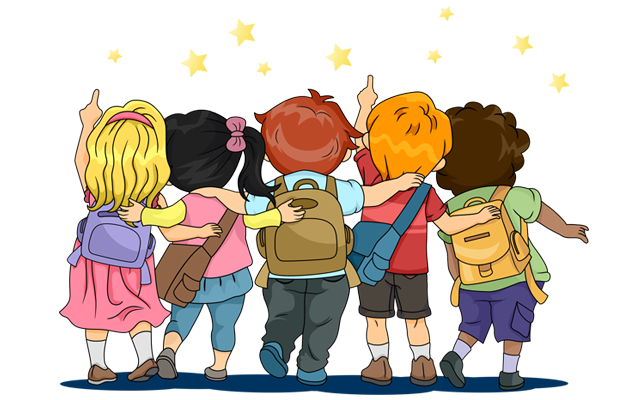
\includegraphics[width=0.8\linewidth]{G7_Modyul_Images/backpack-child-clip-art-student-5a6c1497326783_2412392815170325992065.png}
		\end{center}
	Sa panahon ng pagdadalaga o pagbibinata, may walong inaasahang kakayahan at kilos na dapat malinang ayon kay \textbf{Havighurst }(Hurlock, 1982, p.11). Ang mga ito ay ang mga sumusunod:\\
   \textbf{ 1.} pagtatamo ng bago at ganap na pakikipag-ugnayan (more mature relations) sa mga kasing edad\\
    \textbf{2.} pagtanggap ng papel sa lipunan na angkop sa babae o lalaki\\
    \textbf{3.} pagtanggap sa mga pagbabago sa katawan at paglapat ng tamang pamamahala sa mga ito\\
    \textbf{4.} pagnanais at pagtamo ng mapanagutang asal sa pakikipagkapwa\\
    \textbf{5.} pagkakaroon ng kakayahang makagawa ng maingat na pagpapasya\\
    \textbf{6.} paghahanda para sa paghahanapbuhay\\
    \textbf{7.} paghahanda para sa pag-aasawa at pagpapamilya\\
    \textbf{8.} pagkakaroon ng mga pagpapahalaga (values) na gabay sa mabuting asal\\

% Other news (3)
% -----
\NewsItem{\textbf{Paglalarawan ng mga Inaasahang Kakayahan at Kilos}}
	\textbf{1. Pagtatamo ng bago at ganap na pakikipag-ugnayan \textit{(more mature relations)} sa mga kasingedad.}\\
	\begin{center}
			
\includegraphics[width=0.8\linewidth]{G7_Modyul_Images/child-youth-clip-art-happy-talking-kids-5a8a8a9069c803_0378748615190288804333.png}
		\end{center}
	Para sa isang bata, mahalaga ang pagkakaroon ng kalaro dahil ito ang magtuturo sa kaniya ng pakikipag-ugnayan. Ngunit habang lumalaki at nagkakaisip, nababago ang kaniyang pagtingin sa kaniyang kapwa. Nagiging mas malalim ang kanyang pagtingin sa pakikipag-ugnayan. Naghahanap na siya ng mga taong makakasama niya nang mas madalas sa araw-araw, makakasundo sa maraming bagay at ibang gawain. Ang tawag niya rito ay mga \textit{kaibigan.} Sila ang mga taong tumutulong sa kaniya upang matanggap at mapabilang siya sa isang pangkat na labas sa kaniyang pamilya. Ngunit mahalagang maunawaan niya na may tungkulin siya sa paghubog ng isang maayos at ganap na pakikipag-ugnayan.\\
	Sa puntong ito, makatutulong sa iyo ang sumusunod na hakbang:\\
		    \textbf{a. Alamin mo kung ano talaga ang iyong nais.} Kailangang malinaw sa iyo kung ano ang iyong nais sa isang pakikipag-ugnayan.\\
		    \textbf{b. Ipakita ang tunay na ikaw.} Huwag kang mahiyang ipakita sa kanila ang tunay mong pagkatao. Matuto kang ipahayag ang iyong pagtutol sa mga bagay na labag sa kabutihan. Ang pagtanggap ng iyong mga kaibigan sa aspektong ito ng iyong pagkatao ay nangangahulugang pagtanggap sa tunay na ikaw nang walang halong pagkukunwari.
		\begin{center}
			
\includegraphics[width=0.8\linewidth]{G7_Modyul_Images/domino-mask-masquerade-ball-carnival-5aeece51301706_949867871525599825197.png}
		\end{center}
		    \textbf{c. Panatilihing bukas ang komunikasyon.} Ang pagbabahagi ng iyong nararamdaman, ninanais, mga plano, mga takot, kasiyahan at iba pa ay mahalaga tungo sa isang ganap na pakikipag-ugnayan. Mas makabuluhan ang pakikipag-ugnayan kung walang anumang itinatago sa bawat isa.\\
		\begin{center}
			
\includegraphics[width=0.8\linewidth]{G7_Modyul_Images/international-student-royalty-free-illustration-exchange-of-men-and-women.png}
		\end{center}
		    \textbf{d. Tanggapin ang kapwa at kaniyang tunay na pagkatao.} Ang pakikipag-ugnayan ay walang kondisyon. Mahalagang tanggapin ang isang tao bilang tunay na siya.\\
		    \textbf{e. Panatilihin ang tiwala sa isa't isa.} Kung walang tiwala sa isa't isa, mahina ang pundasyon ng ugnayan. Kung mananatili ang pagtitiwala sa isa't isa, kayang lagpasan ang anumang mga pagsubok sa pakikipag-ugnayan. Kaya lang, iwasang maging masyadong pamilyar sa isa't isa. Ibig sabihin, hindi lahat ng sensitibong bagay sa iyo (tulad ng isang karanasang may negatibong epekto sa iyo) ay dapat mong ibahagi. Baka gamitin ang impormasyon na ito sa ikapapahamak mo balang araw. May kasabihan sa Ingles na \textit{"Familiarity breeds contempt."}\\
		    \textbf{f. Maglaro at maglibang.} Walang pinakamasarap kundi ang maging bata \textit{(childlike)}. Kung minsan sa labis na pagiging seryoso natin sa buhay, nakalilimutan na natin ang halaga ng paminsan-minsang paglalaro at paglilibang na kasama ang mga kaibigan. Sa paraang ito, nakakalimutan natin ang maraming pag-aalala, takot, pagdududa at insekyuridad \textit{(insecurities)}.
		\begin{center}
			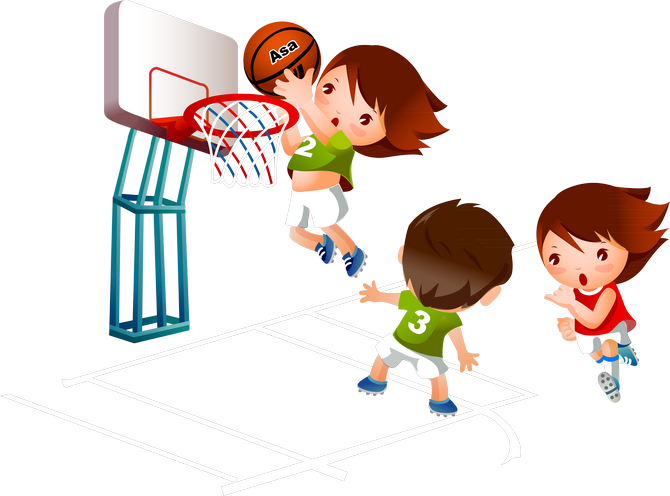
\includegraphics[width=0.8\linewidth]{G7_Modyul_Images/basketball-cartoon-sport-clip-art-kids-playing-basketball-5a96831d00a599_9354601815198134050027.png}
		\end{center}
		\textbf{g. Mahalin mo ang iyong sarili.} Kung hindi mo matututuhang mahalin ang iyong sarili, hindi mo matututuhan ang magpahalaga sa ibang tao.\\
		
\textbf{2. Pagtanggap ng papel sa lipunan na angkop sa babae o lalaki.} Ang mga nagdadalaga o nagbibinata ay bumubuo ng kanilang sariling kahulugan ng pagiging lalaki o babae. Ngunit hindi pa rin naiaalis na ibatay ito sa nakagisnang kultura. Halimbawa, ang lalaki ay malakas, matapang at ang babae naman ay mahina, palaasa. Ang kanilang pagkakaibang biyolohikal ang nagtutulak upang magkaroon ng ganitong pananaw. Ngunit hindi nararapat na lagyan ng hangganan ang kakayahan ng bawat isa batay lamang sa kaniyang katangiang biyolohikal. Sa tulong at paggabay ng mga nakatatanda, kailangang mabigyan ng pagkakataon ang bawat isa na hubugin ang kanilang mga papel sa lipunan bilang lalaki at babae. Halimbawa, kailangan na turuan ang mga lalaki na ipakita ang kanilang tunay na damdamin. Umiyak sila kung kinakailangan sa panahon ng labis na kalungkutan. Kailangang salungatin ang paniniwalang ang umiiyak na lalaki ay labis na mahina.\\

\textbf{3. Pagtanggap sa mga pagbabago sa katawan at paglalapat ng tamang pamamahala sa mga ito.} Sa yugto ng pagdadalaga o pagbibinata, mabilis ang mga pisikal na pagbabago sa katawan kung ihahalintulad sa ibang yugto ng buhay, maliban sa unang dalawang taon ng isang bata. Sa isang binatilyo o dalagita, ang pagkakaiba niya sa iba sa bilis ng paglaki ay maaaring maging dahilan ng insekyuridad \textit{(insecurity)}.\\

\textbf{4. Pagtamo at pagtanggap ng mapanagutang asal sa pakikipagkapwa.} \textit{(Desiring and achieving socially responsible behaviour).} Habang lumilipas ang panahon at ikaw ay nagkakaisip, nakikita mo ang unti-unting paglawak ng mundong iyong ginagalawan. Mula sa iyong tahanan, lumalawak ito habang nadaragdagan ang iyong edad. Ang pagiging mapanagutan sa pakikipagkapwa ay lagpas na sa simpleng paggalang sa kapwa. Ito ay pag-unawa at pagbibigay-halaga sa katotohanang hindi nabubuhay ang tao para lamang sa kaniyang sarili. Kailangan natin ang ibang tao upang tunay na makita ang ganda at halaga ng buhay. Para sa isang nagdadalaga o nagbibinata, mahalaga ito upang tunay na makilala ang kaniyang pagkatao, upang matukoy kung saan siya nababagay sa lipunan at upang mabuo ang kaniyang tiwala na makibahagi sa anumang gawain o trabaho.\\

\textbf{5. Pagkakaroon ng kakayahang makagawa ng maingat na pagpapasiya.} Ang isang bata ay labis na palaasa sa kaniyang mga magulang. Hindi siya makapagpapasiya kung hindi nasa ilalim ng kanilang paggabay. Makararamdam lamang siya ng seguridad kung alam niyang nariyan sila upang suportahan at tulungan siya. Sa yugto ng pagdadalaga o pagbibinata, kinakailangang matutong linangin ang kakayahan sa maingat na pagpapasya. Mahalagang sumangguni sa mga nakatatanda o awtoridad na higit na may alam sa mabuting pamumuhay (tulad ng magulang o kapatid) sa mga pasiyang gagawin; ngunit sanayin na ang sarili na piliin ang patungo sa kabutihan - yaong makabubuti sa sarili, sa kapwa, pamayanan at sa bansa.\\
\begin{center}
			
\includegraphics[width=0.8\linewidth]{G7_Modyul_Images/daily-lives-of-high-school-boys-anime-nichijou-hid-5af7edf2166904_1087153315261977460918.png}
		\end{center}
\textbf{6. Paghahanda para sa paghahanapbuhay.} Sa ating lipunan, iminumulat ang mata ng mga nagdadalaga o nagbibinata na matutuhan ang mga kakayahan na kailangan upang makakuha ng magandang hanapbuhay sa hinaharap. Makatutulong sa iyo ang sumusunod:\\
a. Kilalanin ang iyong mga talento, hilig, kalakasan at kahinaan.\\
b. Makipagkaibigan at lumahok sa iba't ibang gawain sa paaralan (extra curricular activities).\\
c. Magkaroon ng plano sa kursong akademiko o teknikal-bokasyonal na ibig kunin sa hinaharap.\\
d. Sumangguni sa mga matagumpay na kakilala na may hanapbuhay o negosyo upang magtanong tungkol sa mga ginagawa nila sa nasabing hanapbuhay o negosyo\\
e. Hubugin ang tiwala sa sarili at ang kakayahan sa pagpapasiya\\
f. Hingin ang payo ng mga magulang sa pagpili ng angkop na kurso para sa iyo.\\
Ang iba pang mga kakayahan na makatutulong sa iyo ay mas malawak na tatalakayin sa susunod na mga aralin.\\

\textbf{7. Paghahanda para sa pag-aasawa at pagpapamilya.} Kasama sa mga kakayahan at dapat gawin na lilinangin sa isang nagdadalaga o nagbibinata ay ang mapaghandaan ang pag-aasawa at pagpapamilya. Ngunit mahalagang maunawaan na ganap lamang na matatamo ang kakayahang ito sa huling yugto ng pagdadalaga o pagbibinata at sa maagang yugto ng pagtanda (adulthood). Sa kasalukuyang yugto ng iyong buhay, ituon mo muna ang iyong pansin sa pag-aaral upang makamit ang iyong mga pangarap at mithiin.\\

\textbf{8. Pagkakaroon ng mga pagpapahalaga (values) na gabay sa mabuting asal.} Sa yugto ng pagdadaaga o pagbibinata, kailangang mahubog ang iyong mga pagpapahalaga. Bibigyang-tuon sa mga susunod na aralin ang pagtalakay sa paksang ito.\\

\textit{Ang pinakamahalaga, kailangang buong-buo ang iyong tiwala sa iyong sarili at sa iyong mga kakayahan. Mahalaga ito upang mapagtagumpayan mo ang anumang hamon na iyong kakaharapin sa yugto ng pagdadalaga o pagbibinata. Ang pagkakaroon ng tiwala sa sarili ay nangangahulugan ng pagkakaroon ng positibong pagtingin sa iyong mga kakayahan. Hindi ka nalilimitahan ng mga negatibong pag-iisip na madalas ay hindi naman makatotohanan.}\\

% Other news (3)
% -----

\NewsItem{\textbf{Pagkakaroon ng Positibong Pananaw at Damdamin Tungkol sa iyong Sarili}}

Sa pamamagitan ng positibong pag-iisip, mapatataas mo ang iyong tiwala sa sarili at magkakaroon ka ng positibong pananaw at damdamin tungkol sa iyong sarili. Makatutulong sa iyo ang sumusunod:\\

\textbf{a. Hayaang mangibabaw ang iyong mga kalakasan.} Mag-isip ng positibo sa lahat ng iyong mga ginagawa at purihin ang sarili dahil sa iyong pagsisikap. Hindi ito nangangahulugan na hindi mo na bibigyan ng tuon ang iyong kahinaan, ngunit hindi nararapat na malimitahan ng iyong mga kahinaan ang iyong mga kalakasan.\\

\textbf{b. Huwag matakot na harapin ang mga bagong hamon.} Ang mga bagong hamon ay pagkakataon upang iyong mapataas ang tiwala sa sarili. Hindi mo nararapat isipin ang takot ng pagkabigo o ang tagumpay ng pagwawagi. Isipin mo na lamang na sa tuwing may gagawin kang bago: (1) nabibigyan ka ng pagkakataon na magsikap upang matamo ang tagumpay, (2) napatataas mo ang iyong tiwala sa sarili, at (3) mas nakikilala at natatanggap mo ang iyong sarili.\\

\textbf{c. Palaging maging positibo sa iyong mga pag-iisip.} Lahat ng mga karanasan, positibo man o hindi, ay may mabuting ibubunga tungo sa pag-unlad ng iyong pagkatao. Palaging ipaalala sa sarili na hindi mo man kayang gawin ang lahat ng bagay nang perpekto, makatutulong naman ang mga ito upang unti-unting umunlad ang iyong pananaw sa bawat araw.\\

\textbf{d. Isipin mo ang iyong mga kakayahan para sa iyong sarili: huwag palaging umasa sa opinyon ng ibang tao,} lalo na ang pagtataya sa iyong mga kabiguan at tagumpay. Mas makatutulong kung mapauunlad mo ang iyong kakayahan sa pagsusuri at pagtataya ng iyong sarili. Isa itong malaking hakbang sa pagpapataas ng iyong tiwala sa sarili.\\

Mahirap ang pinagdaraanan mo, ngunit tandaan na hindi ka nag-iisa. Lahat ng nagdadalaga o nagbibinata ay may katulad na pinagdaraanan. Maiiba lamang ito ayon sa kung paano mo isinabuhay ang mga kakayahan at kilos na kinakailangan para mas mapaunlad mo ang iyong sarili at ang iyong pagkatao.\\

Ngayon, nakahanda ka na ba sa pagtataya ng iyong sarili kaugnay ng konseptong iyong natutuhan sa aralin sa modyul na ito?
\end{multicols*}
% -----
\end{document} 
